         \chapter{Electrostatics}
    \setcounter{figure}{1}
    \setcounter{subfigure}{1}
    \label{464e844ca5615087ea89d9d95dd9a43a}
    
    
    
    
       
         \section{ Introduction and key concepts}
    \nopagebreak
            \label{m38780} $ \hspace{-5pt}\begin{array}{cccccccccccc}   
\includegraphics[width=0.75cm]{col11305.imgs/summary_fullmarks.png} &   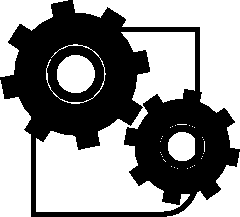
\includegraphics[width=0.75cm]{col11305.imgs/summary_simulation.png} &   \end{array} $ \hspace{2 pt}\raisebox{-5 pt}{} {(section shortcode: P10071 )} \par 
    
    
    
    
    
    
  
    \label{m38780*cid2}
            \subsection{ Introduction}
            \nopagebreak
            
      
      \label{m38780*id200254}Electrostatics is the study of electric charge which is static (not moving). In this chapter we will look at some of the basic principle of electric charge as well as the principle of conservation of charge. \par 
    
    \label{m38780*cid3}
            \subsection{ Two kinds of charge}
            \nopagebreak
            
      
      \label{m38780*id200267}All objects surrounding us (including people!) contain large amounts of electric charge. There
are two types of electric charge: \textbf{positive} charge and \textbf{negative} charge.
If the same amounts
of negative and positive charge are brought together, they neutralise each other and there
is \textsl{no net charge}. \textbf{Neutral} objects are objects which contain equal amouts of positive
and negative charges. However, if there is a little bit more of one type of charge than the other on the
object then the object is said to be \textbf{electrically charged}. The picture below shows
what the distribution of charges might look like for a neutral, positively charged and
negatively charged object.\par 
      \label{m38780*id200640}
        
    \setcounter{subfigure}{0}


	\begin{figure}[H] % horizontal\label{m38780*id200643}
    \begin{center}
    \label{m38780*id200643!!!underscore!!!media}\label{m38780*id200643!!!underscore!!!printimage}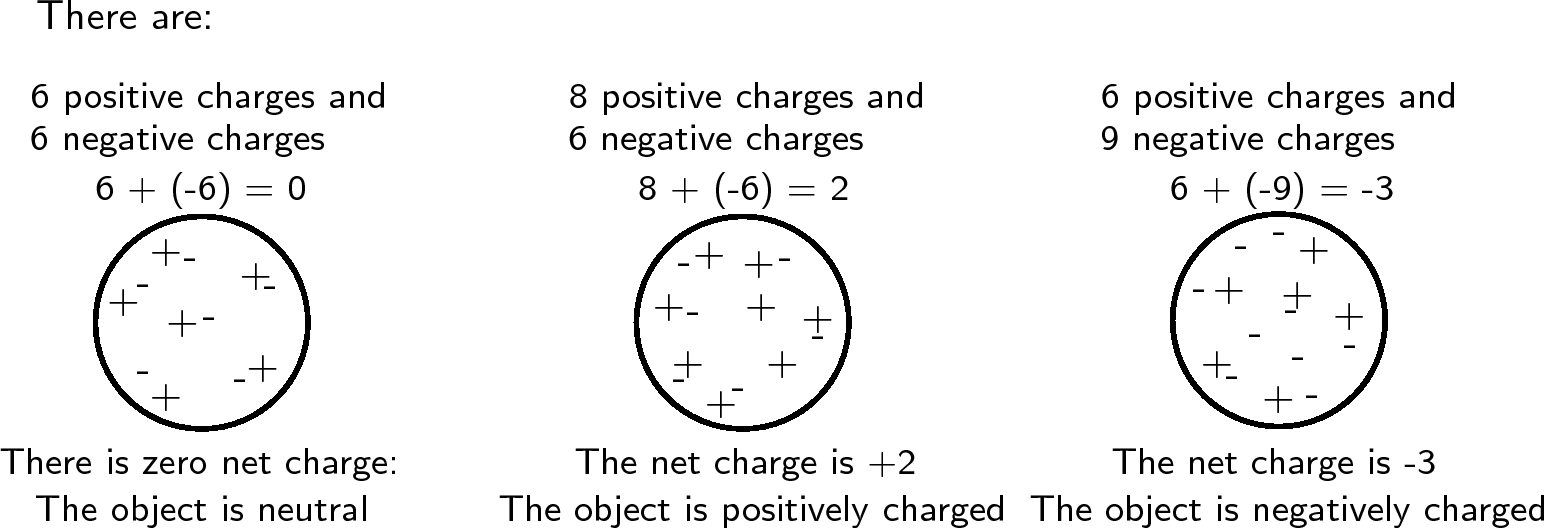
\includegraphics[width=300px]{col11305.imgs/m38780_PG10C8_001.png} % m38780;PG10C8\_001.png;;;6.0;8.5;
        
      \vspace{2pt}
    \vspace{.1in}
    
    \end{center}

 \end{figure}   

    \addtocounter{footnote}{-0}
    
      \par \label{m38780*eip-429}To complete: electrically negative objects have an electron excess and positively charged objects have an electron deficiency.\par 
    
    
    \label{m38780*cid5}
            \subsection{ Tribo-Electric Charging}
            \nopagebreak
            \label{m38780*id200729}Objects may become charged in many ways, including by contact with or being rubbed by other objects. This means that they can gain extra negative or positive charge. For example, charging happens
when you rub your feet against the carpet. When you
then touch something metallic or another person, you feel a shock as
the excess charge that you have collected is \textsl{discharged}.\par 
\label{m38780*notfhsst!!!underscore!!!id106}
\begin{tabular}{cc}
	   \hspace*{-50pt}\raisebox{-8 mm}{ 
\includegraphics[width=0.5in]{col11305.imgs/pstip2.png}  }& 

	\begin{minipage}{0.85\textwidth}
	\begin{note}
      {tip: }Charge, like energy, cannot be created or destroyed. We say
that charge is \textbf{conserved}.
	\end{note}
	\end{minipage}
	\end{tabular}
	\par
      
\label{m38780*id200752}When you rub your feet
against the carpet, negative charge is transferred to you
from the carpet. The carpet will then become positively
charged by the \textsl{same amount}.\par 
      \label{m38780*id200762}Another example is to take two \textsl{neutral} objects such as a plastic ruler and a cotton cloth (handkerchief). To begin, the two objects are neutral (i.e. have the same amounts of positive and negative charge).\par 
      \label{m38780*id200774}
        
    \setcounter{subfigure}{0}


	\begin{figure}[H] % horizontal\label{m38780*id200777}
    \begin{center}
    \label{m38780*id200777!!!underscore!!!media}\label{m38780*id200777!!!underscore!!!printimage}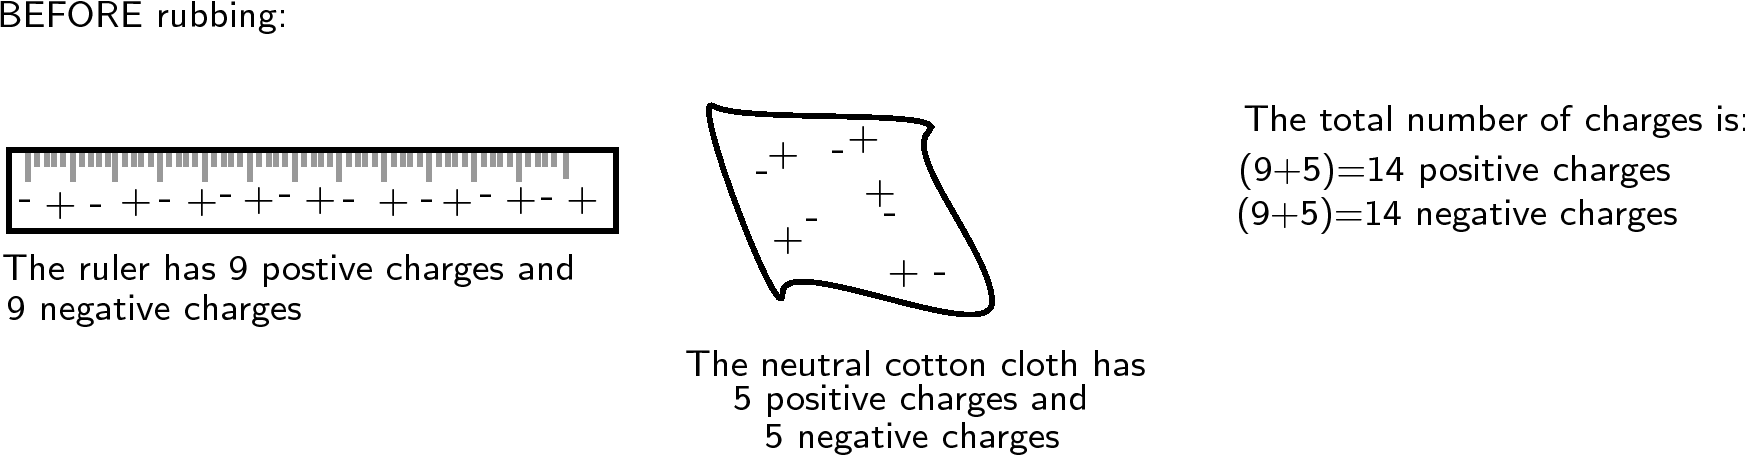
\includegraphics[width=300px]{col11305.imgs/m38780_PG10C8_002.png} % m38780;PG10C8\_002.png;;;6.0;8.5;
        
      \vspace{2pt}
    \vspace{.1in}
    
    \end{center}

 \end{figure}   

    \addtocounter{footnote}{-0}
    
      \par 
      \label{m38780*id200783}Now, if the cotton cloth is used to rub the ruler, negative charge
is transferred \textsl{from} the cloth \textsl{to} the ruler.
The ruler is now \textsl{negatively} charged (i.e. has an excess of electrons) and the cloth is \textsl{positively} charged (i.e. is electron deficient).
If you count up all the positive and negative charges at the beginning and the end, there are still the same amount. i.e. total charge has been \textsl{conserved}!\par 
      \label{m38780*id200814}
        
    \setcounter{subfigure}{0}


	\begin{figure}[H] % horizontal\label{m38780*id200819}
    \begin{center}
    \label{m38780*id200819!!!underscore!!!media}\label{m38780*id200819!!!underscore!!!printimage}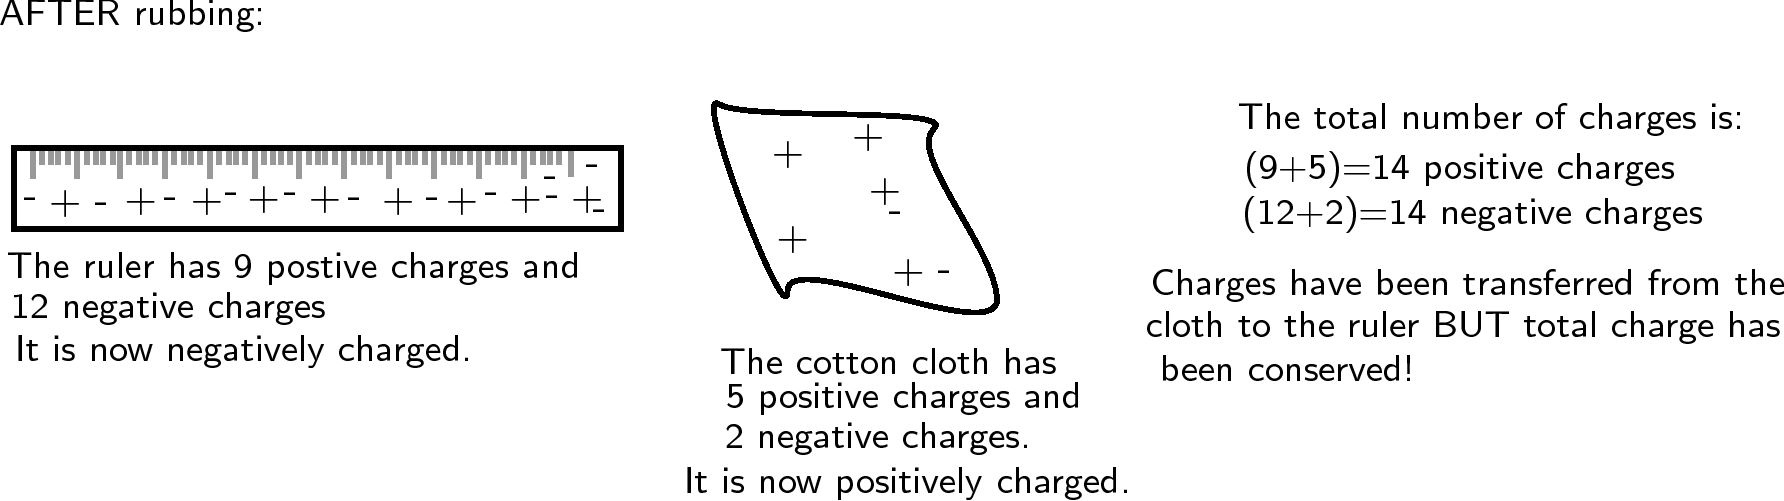
\includegraphics[width=300px]{col11305.imgs/m38780_PG10C8_003.png} % m38780;PG10C8\_003.png;;;6.0;8.5;
        
      \vspace{2pt}
    \vspace{.1in}
    
    \end{center}

 \end{figure}   

    \addtocounter{footnote}{-0}
    
      \par 
      \label{m38780*id200825}Note that in this example the numbers are made up to be easy to calculate. In the real world only a tiny fraction of the charges would move from one object to the other, but the total charge would still be conserved.\par \label{m38780*eip-600}The following simulation will help you understand what happens when you rub an object against another object.\newline
     run demo\footnote{http://phet.colorado.edu/sims/balloons/balloons\_en.jnlp}
        

    \setcounter{subfigure}{0}


	\begin{figure}[H] % horizontal\label{m38780*id11328}
    \begin{center}
    \label{m38780*id11328!!!underscore!!!media}\label{m38780*id11328!!!underscore!!!printimage}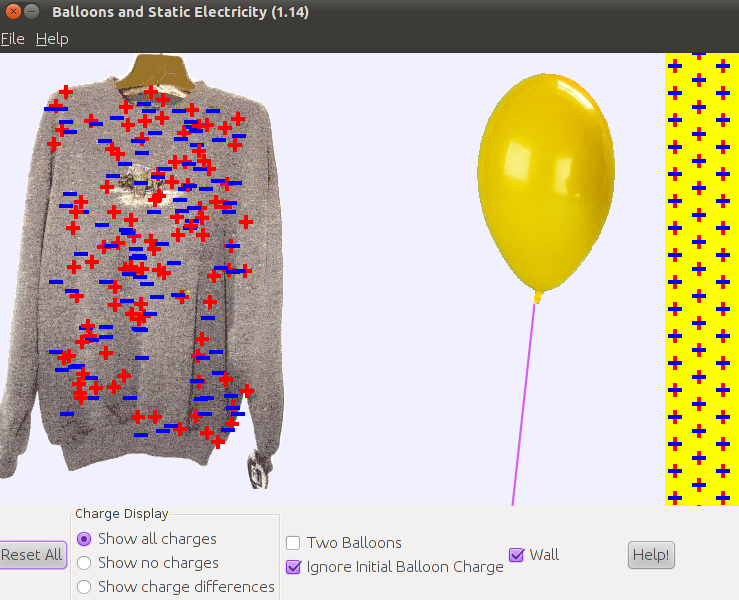
\includegraphics{col11305.imgs/m38780_phet1.png} % m38780;phet1.png;;;6.0;8.5;
        
      \vspace{2pt}
    \vspace{.1in}
    
    \end{center}

 \end{figure}   

    \addtocounter{footnote}{-0}
    \par \label{m38780*eip-567}
\begin{tabular}{cc}
	\hspace*{-50pt}\raisebox{-8 mm}{\hspace{-0.2in}
\includegraphics[width=0.75in]{col11305.imgs/psfact2.png} } & 

	\begin{minipage}{0.85\textwidth}
	\begin{note}
      {note: }The process of materials becoming charged when they come into contact with other materials is known as tribo-electric charging. Materials can be arranged in a tribo-electric series according to whether they are more positive or more negative. This tribo-electric series can allow us to determine whether one material is likely to become charged from another material. For example, amber is more negative than wool and so if a piece of wool is rubbed against a piece of amber then the amber will become negatively charged.
	\end{note}
	\end{minipage}
	\end{tabular}
	\par
      
    
    \label{m38780*cid6}
            \subsection{ Force between Charges}
            \nopagebreak
            \label{m38780*id200840}The force exerted by non-moving (static) charges on each other is called the \textbf{electrostatic force.} The electrostatic force between:\par 
      \label{m38780*id200849}\begin{itemize}[noitemsep]
            \label{m38780*uid1}\item \textbf{like} charges is \textbf{repulsive}\label{m38780*uid2}\item \textbf{opposite} (unlike) charges is \textbf{attractive}.
\end{itemize}
        
      \label{m38780*id200894}In other words, like charges repel each other while opposite
charges attract each other. This is different to the gravitational force which is only attractive.\par 
      \label{m38780*id200898}
    \setcounter{subfigure}{0}


	\begin{figure}[H] % horizontal\label{m38780*id200901}
    \begin{center}
    \label{m38780*id200901!!!underscore!!!media}\label{m38780*id200901!!!underscore!!!printimage}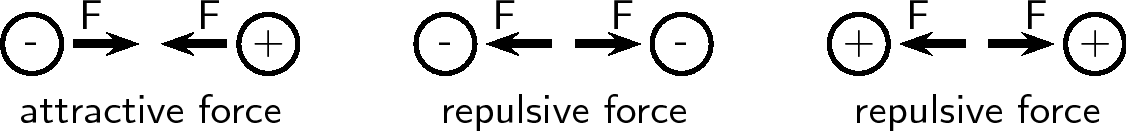
\includegraphics[width=300px]{col11305.imgs/m38780_PG10C8_004.png} % m38780;PG10C8\_004.png;;;6.0;8.5;
        
      \vspace{2pt}
    \vspace{.1in}
    
    \end{center}

 \end{figure}   

    \addtocounter{footnote}{-0}
    
      \par 
      \label{m38780*id200907}The \textsl{closer} together the charges are, the \textsl{stronger} the electrostatic force between them.\par 
      \label{m38780*id200921}
        
    \setcounter{subfigure}{0}


	\begin{figure}[H] % horizontal\label{m38780*id200924}
    \begin{center}
    \label{m38780*id200924!!!underscore!!!media}\label{m38780*id200924!!!underscore!!!printimage}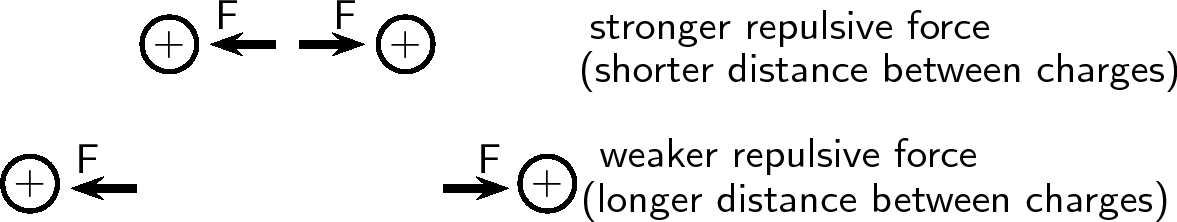
\includegraphics[width=300px]{col11305.imgs/m38780_PG10C8_005.png} % m38780;PG10C8\_005.png;;;6.0;8.5;
        
      \vspace{2pt}
    \vspace{.1in}
    
    \end{center}

 \end{figure}   

    \addtocounter{footnote}{-0}
    
      \par 
\label{m38780*secfhsst!!!underscore!!!id162}
            \subsubsection{  Experiment : Electrostatic Force }
            \nopagebreak
            
      \label{m38780*id200937}You can easily test that
like charges repel and unlike charges attract each other by doing a very
simple experiment.\par 
      \label{m38780*id200944}Take a glass rod and rub it with a piece of silk, then hang it from its middle with a piece string so that it is free to move. If you then bring another glass rod which you
have also charged in the same way next to it, you will see the rod
on the string turn \textsl{away} from the rod in your hand i.e. it
is \textbf{repelled}. If, however, you take a plastic rod, rub it
with a piece of fur and then bring it close to the rod on the
string, you will see the rod on the string turn \textsl{towards} the
rod in your hand i.e. it is \textbf{attracted}.\par 
      \label{m38780*id200971}
        
    \setcounter{subfigure}{0}


	\begin{figure}[H] % horizontal\label{m38780*id200974}
    \begin{center}
    \label{m38780*id200974!!!underscore!!!media}\label{m38780*id200974!!!underscore!!!printimage}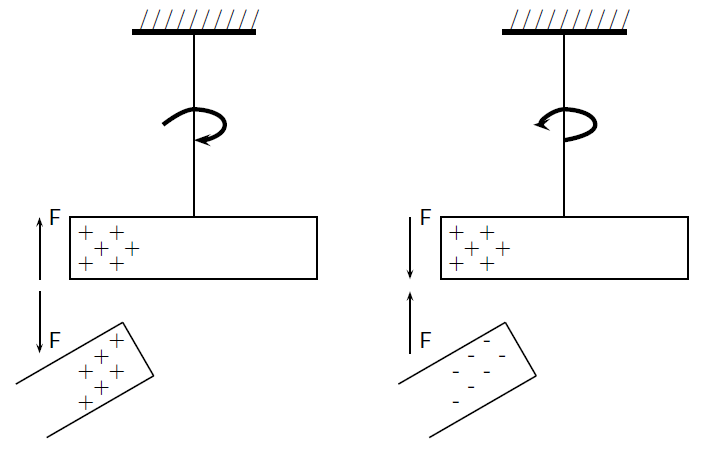
\includegraphics[width=300px]{col11305.imgs/m38780_PG10C8_006.png} % m38780;PG10C8\_006.png;;;6.0;8.5;
        
      \vspace{2pt}
    \vspace{.1in}
    
    \end{center}

 \end{figure}   

    \addtocounter{footnote}{-0}
    
      \par 
      \label{m38780*id200980}This happens because when you rub the glass with silk,
tiny amounts of negative charge are transferred from the glass
onto the silk, which causes the glass to have less negative charge
than positive charge, making it \textbf{positively charged}. When
you rub the plastic rod with the fur, you transfer tiny amounts of
negative charge onto the rod and so it has more negative charge
than positive charge on it, making it \textbf{negatively charged}.
 \par 

\label{m38780*secfhsst!!!underscore!!!id190}\vspace{.5cm} 
      
      \noindent
      \hspace*{-30pt}
\includegraphics[width=0.5in]{col11305.imgs/pspencil2.png}   \raisebox{25mm}{   
      \begin{mdframed}[linewidth=4, leftmargin=40, rightmargin=40]  
      \begin{exercise}
    \noindent\textbf{Exercise 15.1:  Application of electrostatic forces }
      \label{m38780*probfhsst!!!underscore!!!id191}
      \label{m38780*id201015}Two charged metal spheres hang from strings and are free to move as shown in the picture below. The right hand sphere is positively charged. The charge on the left hand sphere is unknown.\par 
      \label{m38780*id201022}
        
    \setcounter{subfigure}{0}


	\begin{figure}[H] % horizontal\label{m38780*id201025}
    \begin{center}
    \label{m38780*id201025!!!underscore!!!media}\label{m38780*id201025!!!underscore!!!printimage}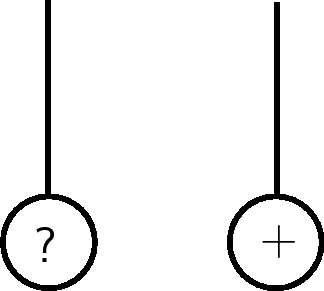
\includegraphics[width=300px]{col11305.imgs/m38780_PG10C8_007.png} % m38780;PG10C8\_007.png;;;6.0;8.5;
        
      \vspace{2pt}
    \vspace{.1in}
    
    \end{center}

 \end{figure}   

    \addtocounter{footnote}{-0}
    
      \par 
      \label{m38780*id201031}The left sphere is now brought close to the right sphere.\par 
      \label{m38780*id201034}\begin{enumerate}[noitemsep, label=\textbf{\arabic*}. ] 
            \leftskip=20pt\rightskip=\leftskip\label{m38780*uid3}\item If the left hand sphere swings towards the right hand sphere, what can you say about the charge on the left sphere and why?
\label{m38780*uid4}\item If the left hand sphere swings away from the right hand sphere, what can you say about the charge on the left sphere and why?
\end{enumerate}
        
      
      \vspace{5pt}
      \label{m38780*solfhsst!!!underscore!!!id210}\noindent\textbf{Solution to Exercise } \label{m38780*listfhsst!!!underscore!!!id210}\begin{enumerate}[noitemsep, label=\textbf{Step} \textbf{\arabic*}. ] 
            \leftskip=20pt\rightskip=\leftskip\item  
      \label{m38780*id201084}In the first case, we have a sphere with positive charge which is \textsl{attracting} the left charged sphere. We need to find the charge on the left sphere.\par 
      \item  
      \label{m38780*id201097}We are dealing with electrostatic forces between charged objects. Therefore, we know that \textsl{like} charges \textsl{repel} each other and \textsl{opposite} charges \textsl{attract} each other.\par 
      \item  
      \label{m38780*id201126}\begin{enumerate}[noitemsep, label=\textbf{\alph*}. ] 
            \leftskip=20pt\rightskip=\leftskip\label{m38780*uid5}\item In the first case, the positively charged sphere is attracting the left sphere. Since an electrostatic force between unlike charges is attractive, the left sphere must be \textsl{negatively} charged.
\label{m38780*uid6}\item In the second case, the positively charged sphere repels the left sphere. Like charges repel each other. Therefore, the left sphere must now also be \textsl{positively} charged.
\end{enumerate}
        
      
      \end{enumerate}
         

    \end{exercise}
    \end{mdframed}
    }
    \noindent
  

\label{m38780*notfhsst!!!underscore!!!id250}
\begin{tabular}{cc}
	\hspace*{-50pt}\raisebox{-8 mm}{\hspace{-0.2in}
\includegraphics[width=0.75in]{col11305.imgs/psfact2.png} } & 

	\begin{minipage}{0.85\textwidth}
	\begin{note}
      {note: }The word 'electron' comes from the Greek word for amber. The
ancient Greeks observed that if you rubbed a piece of amber, you
could use it to pick up bits of straw.

	\end{note}
	\end{minipage}
	\end{tabular}
	\par
      \label{m38780*eip-430}
            \subsubsection{ Polarisation}
            \nopagebreak
            \label{m38780*id201876}Unlike conductors, the electrons in insulators (non-conductors) are bound to the atoms of the
insulator and cannot move around freely through the material. However, a charged object can still
exert a force on a neutral insulator due to a phenomenon called \textbf{polarisation}.\par 
        \label{m38780*id201887}If a positively charged rod is
brought close to a neutral insulator such as polystyrene, it can attract the bound electrons
to move round to the
side of the atoms which is closest to the rod and cause the positive nuclei to move slightly
to the opposite side of the atoms. This process is called \textsl{polarisation}. Although
it is a very small (microscopic) effect, if there are many atoms and the polarised object is
light (e.g. a small polystyrene ball), it can add up to enough force to cause the object to be attracted onto the
charged rod. Remember, that the polystyrene
is \textsl{only} polarised, \textsl{not charged.}
The polystyrene ball is still neutral since no charge was added or removed from it.
The picture shows
a not-to-scale view of the polarised atoms in the polystyrene ball:\par 
        \label{m38780*id201914}
    \setcounter{subfigure}{0}


	\begin{figure}[H] % horizontal\label{m38780*id201917}
    \begin{center}
    \label{m38780*id201917!!!underscore!!!media}\label{m38780*id201917!!!underscore!!!printimage}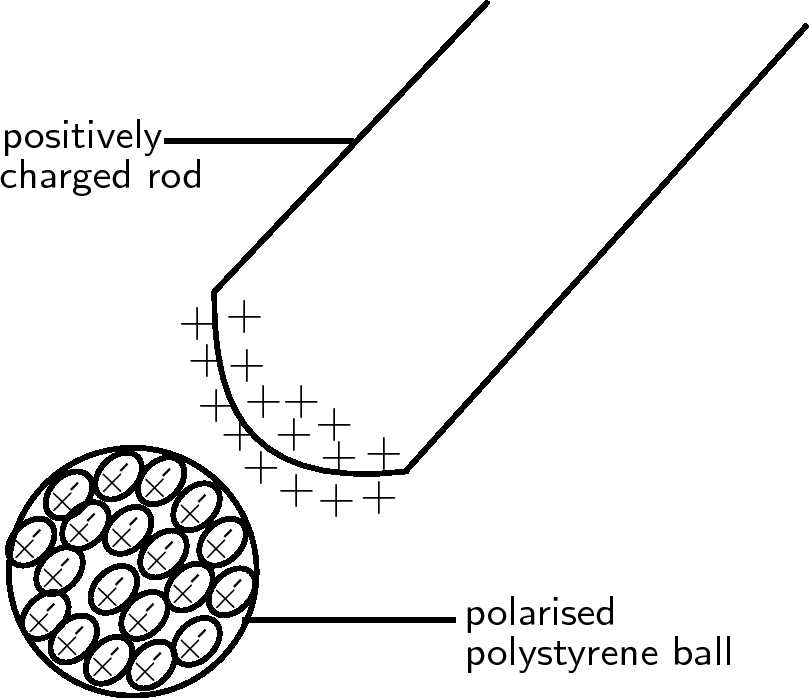
\includegraphics{col11305.imgs/m38780_PG10C8_011.png} % m38780;PG10C8\_011.png;;;6.0;8.5;
        
      \vspace{2pt}
    \vspace{.1in}
    
    \end{center}

 \end{figure}   

    \addtocounter{footnote}{-0}
    
        \par 
        \label{m38780*id201923}Some materials are made up of molecules which are already polarised.
These are molecules which have
a more positive and a more negative side but are still neutral overall.
Just as a polarised polystyrene ball can be attracted to a charged rod, these materials
are also affected if brought close to a charged object.\par 
        \label{m38780*id201929}Water is an example of a substance which is made of polarised molecules.
If a positively charged rod is brought close to a stream of water, the molecules can rotate
so that the negative sides all line up towards the rod.
The stream of water will then be attracted to the rod since opposite charges attract.\par 
      
    \label{m38780*eip-275}
            \subsection{ Conservation of Charge}
            \nopagebreak
            \label{m38780*eip-506}The principle of conservation of charge states that the net charge of an isolated system remains constant during any physical process, e.g. when two charges make contact and are separated again.\par 

  \label{m38780**end}
          
         \section{ Conductors and insulators}
    \nopagebreak
            \label{m38781} $ \hspace{-5pt}\begin{array}{cccccccccccc}   
\includegraphics[width=0.75cm]{col11305.imgs/summary_fullmarks.png} &   
\includegraphics[width=0.75cm]{col11305.imgs/summary_video.png} &   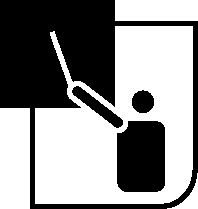
\includegraphics[width=0.75cm]{col11305.imgs/summary_presentation.png} &   \end{array} $ \hspace{2 pt}\raisebox{-5 pt}{} {(section shortcode: P10072 )} \par 
    
    
    
    
    
    
  
    \label{m38781*cid7}
            \subsection{ Conductors and insulators}
            \nopagebreak
            \label{m38781*id201248}All atoms are electrically neutral i.e. they have the same amounts of negative and positive
charge inside them. By convention, the electrons carry negative charge and the protons carry
positive charge.
The basic unit of charge, called the elementary charge, \textsl{e}, is
the amount of charge carried by one electron.\par 
      \label{m38781*eip-517}The charge on a single electron is \begin{math}{q}_{e}=1,6x{10}^{-19}\phantom{\rule{2pt}{0ex}}\mathrm{C}\end{math}. All other charges in the universe consist of an interger multiple of this charge (i.e. \begin{math}\mathrm{Q}={\mathrm{nq}}_{e}\end{math}). This is known as charge quantisation.
\par \label{m38781*id201259}All the matter and materials on earth are made up of atoms.
Some materials allow electrons to move relatively freely
through them (e.g. most metals, the human body).
These materials are called \textbf{conductors}.\par 
      \label{m38781*id201271}Other materials do not allow the charge carriers, the electrons, to move
through them (e.g. plastic, glass).
The electrons are bound to the atoms in the material. These materials are called
\textbf{non-conductors} or \textbf{insulators}.\par 
      \label{m38781*id201289}If an excess of charge is placed on an insulator, it will stay
where it is put and there will be a concentration of charge in
that area of the object. However, if an excess of charge is placed
on a conductor, the like charges will repel each other
and spread out over the outside surface of the object. When two conductors
are made to touch, the total charge on them is shared between the
two. If the two conductors are identical, then each conductor will
be left with half of the total charge.\par 
\label{m38781*eip-536}
\begin{tabular}{cc}
	\hspace*{-50pt}\raisebox{-8 mm}{\hspace{-0.2in}
\includegraphics[width=0.75in]{col11305.imgs/psfact2.png} } & 

	\begin{minipage}{0.85\textwidth}
	\begin{note}
      {note: }\label{m38781*id201187}The electrostatic force determines the
arrangement of charge on the surface of conductors. This is possible because charges can move inside a conductive material. When we place
a charge on a spherical conductor the repulsive forces between the
individual like charges cause them to spread uniformly over the
surface of the sphere. However, for conductors with non-regular
shapes, there is a concentration of charge near the point or points
of the object. Notice in Figure~15.10 that we show a concentration of charge with more \begin{math}-\end{math} or + signs, while we represent uniformly spread charges with uniformly spaced \begin{math}-\end{math} or + signs.\par 
      \label{m38781*id201196}
        
    \setcounter{subfigure}{0}


	\begin{figure}[H] % horizontal\label{m38781*id201199}
    \begin{center}
    \label{m38781*id201199!!!underscore!!!media}\label{m38781*id201199!!!underscore!!!printimage}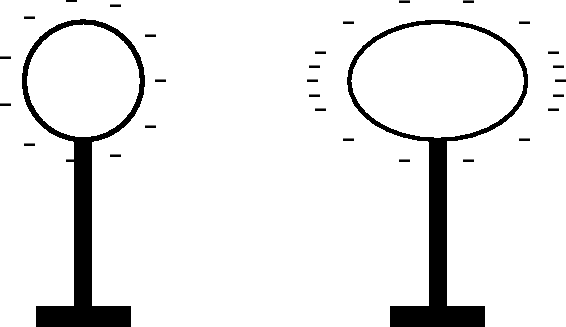
\includegraphics[width=300px]{col11305.imgs/m38781_PG10C8_008.png} % m38781;PG10C8\_008.png;;;6.0;8.5;
        
      \vspace{2pt}
    \vspace{.1in}
    
    \end{center}

 \end{figure}   

    \addtocounter{footnote}{-0}
    
      \par 
      \label{m38781*id201205}This collection of charge can actually allow charge to leak off
the conductor if the point is sharp enough. It is for this reason
that buildings often have a lightning rod on the roof to remove
any charge the building has collected. This minimises the
possibility of the building being struck by lightning. This
``spreading out'' of charge would not occur if we were to place
the charge on an insulator since charge cannot move in
insulators. \par 
	\end{note}
	\end{minipage}
	\end{tabular}
	\par
      \label{m38781*eip-509}
\begin{tabular}{cc}
	\hspace*{-50pt}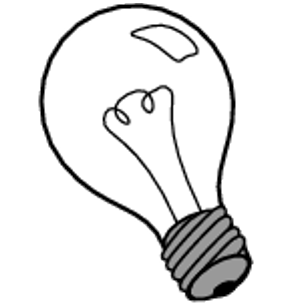
\includegraphics[width=0.5in]{col11305.imgs/psbulb2.png}  & 

	\begin{minipage}{0.85\textwidth}
	\begin{note}
      {aside: }The basic unit of charge, namely the
elementary charge is carried by the
electron (equal to 1.602\begin{math}\ensuremath{\times}{10}^{-19}\end{math} C!). In a conducting material (e.g. copper), when the atoms
bond to form the material, some of the outermost, loosely bound
electrons become detached from the individual atoms and so become
free to move around. The charge carried by these electrons can
move around in the material. In insulators, there are very few, if
any, free electrons and so the charge cannot move around in the
material. 
	\end{note}
	\end{minipage}
	\end{tabular}
	\par
      \label{m38781*eip-841}
\begin{tabular}{cc}
	\hspace*{-50pt}\raisebox{-8 mm}{\hspace{-0.2in}
\includegraphics[width=0.75in]{col11305.imgs/psfact2.png} } & 

	\begin{minipage}{0.85\textwidth}
	\begin{note}
      {note: }In 1909 Robert Millikan and Harvey Fletcher measured the charge on an electron. This experiment is now known as Millikan's oil drop experiment. Millikan and Fletcher sprayed oil droplets into the space between two charged plates and used what they knew about forces and in particular the electric force to determine the charge on an electron.
	\end{note}
	\end{minipage}
	\end{tabular}
	\par
      
\label{m38781*secfhsst!!!underscore!!!id290}\vspace{.5cm} 
      
      \noindent
      \hspace*{-30pt}
\includegraphics[width=0.5in]{col11305.imgs/pspencil2.png}   \raisebox{25mm}{   
      \begin{mdframed}[linewidth=4, leftmargin=40, rightmargin=40]  
      \begin{exercise}
    \noindent\textbf{Exercise 15.2:  Conducting spheres and movement of charge }
      \label{m38781*probfhsst!!!underscore!!!id291}
      \label{m38781*id201351}I have 2 charged metal conducting spheres which are identical except for having different charge. Sphere A has a charge of -5 nC and sphere B has a charge of -3 nC. I then bring the spheres together so that they touch each other. Afterwards I move the two spheres apart so that they are no longer touching.\par 
      \label{m38781*id201359}\begin{enumerate}[noitemsep, label=\textbf{\arabic*}. ] 
            \leftskip=20pt\rightskip=\leftskip\label{m38781*uid7}\item What happens to the charge on the two spheres?
\label{m38781*uid8}\item What is the final charge on each sphere?
\end{enumerate}
        
      
      \vspace{5pt}
      \label{m38781*solfhsst!!!underscore!!!id301}\noindent\textbf{Solution to Exercise } \label{m38781*listfhsst!!!underscore!!!id301}\begin{enumerate}[noitemsep, label=\textbf{Step} \textbf{\arabic*}. ] 
            \leftskip=20pt\rightskip=\leftskip\item  
      \label{m38781*id201406}We have two identical negatively charged conducting spheres which are brought together to touch each other and then taken apart again. We need to explain what happens to the charge on each sphere and what the final charge on each sphere is after they are moved apart.\par 
      \item  
      \label{m38781*id201416}We know that the charge carriers in conductors are free to move around and that charge on a conductor spreads itself out on the surface of the conductor.\par 
      \item  
      \label{m38781*id201425}\begin{enumerate}[noitemsep, label=\textbf{\alph*}. ] 
            \leftskip=20pt\rightskip=\leftskip\label{m38781*uid9}\item When the two conducting spheres are brought together to touch, it is as though they become one single big conductor and the total charge of the two spheres spreads out across the whole surface of the touching spheres. When the spheres are moved apart again, each one is left with half of the total original charge.
\label{m38781*uid10}\item Before the spheres touch, the total charge is: -5 nC + (-3) nC = -8 nC. When they touch they share out the -8 nC across their whole surface. When they are removed from each other, each is left with half of the original charge:
\label{m38781*id201455}\nopagebreak\noindent{}\settowidth{\mymathboxwidth}{\begin{equation}
    \begin{array}{ccc}\hfill \frac{-8\phantom{\rule{4pt}{0ex}}\mathrm{nC}}{2}& =& -4\phantom{\rule{4pt}{0ex}}\mathrm{nC}\hfill \end{array}\tag{15.1}
      \end{equation}
    }
    \typeout{Columnwidth = \the\columnwidth}\typeout{math as usual width = \the\mymathboxwidth}
    \ifthenelse{\lengthtest{\mymathboxwidth < \columnwidth}}{% if the math fits, do it again, for real
    \begin{equation}
    \begin{array}{ccc}\hfill \frac{-8\phantom{\rule{4pt}{0ex}}\mathrm{nC}}{2}& =& -4\phantom{\rule{4pt}{0ex}}\mathrm{nC}\hfill \end{array}\tag{15.1}
      \end{equation}
    }{% else, if it doesn't fit
    \setlength{\mymathboxwidth}{\columnwidth}
      \addtolength{\mymathboxwidth}{-48pt}
    \par\vspace{12pt}\noindent\begin{minipage}{\columnwidth}
    \parbox[t]{\mymathboxwidth}{\large\begin{math}
    \frac{-8\phantom{\rule{4pt}{0ex}}\mathrm{nC}}{2}=-4\phantom{\rule{4pt}{0ex}}\mathrm{nC}\end{math}}\hfill
    \parbox[t]{48pt}{\raggedleft 
    (15.1)}
    \end{minipage}\vspace{12pt}\par
    }% end of conditional for this bit of math
    \typeout{math as usual width = \the\mymathboxwidth}
    
on each sphere.
\end{enumerate}
        
      
      \end{enumerate}
         

    \end{exercise}
    \end{mdframed}
    }
    \noindent
  
      \label{m38781*eip-89}In the previous example we worked out what happens when two identical conductors are allowed to touch. We noticed that if we take two identically sized conducting spheres on insulating stands and bring them together so that they touch, each sphere will have the same final charge. If the initial charge on the first sphere is \begin{math}{Q}_{1}\end{math} and the initial charge on the second sphere is \begin{math}{Q}_{2}\end{math}, then the final charge on the two spheres after they have been brought into contact is:
\label{m38781*id6214}\nopagebreak\noindent{}
\settowidth{\mymathboxwidth}{\begin{equation}
    Q=\frac{{Q}_{1}+{Q}_{2}}{2}\tag{15.2}
      \end{equation}
    }
    \typeout{Columnwidth = \the\columnwidth}\typeout{math as usual width = \the\mymathboxwidth}
    \ifthenelse{\lengthtest{\mymathboxwidth < \columnwidth}}{% if the math fits, do it again, for real
    \begin{equation}
    Q=\frac{{Q}_{1}+{Q}_{2}}{2}\tag{15.2}
      \end{equation}
    }{% else, if it doesn't fit
    \setlength{\mymathboxwidth}{\columnwidth}
      \addtolength{\mymathboxwidth}{-48pt}
    \par\vspace{12pt}\noindent\begin{minipage}{\columnwidth}
    \parbox[t]{\mymathboxwidth}{\large\begin{math}
    Q=\frac{{Q}_{1}+{Q}_{2}}{2}\end{math}}\hfill
    \parbox[t]{48pt}{\raggedleft 
    (15.2)}
    \end{minipage}\vspace{12pt}\par
    }% end of conditional for this bit of math
    \typeout{math as usual width = \the\mymathboxwidth}
    
\par \par
            \label{m38781*eip-918}\vspace{.5cm} 
      
      \noindent
      \hspace*{-30pt}
\includegraphics[width=0.5in]{col11305.imgs/pspencil2.png}   \raisebox{25mm}{   
      \begin{mdframed}[linewidth=4, leftmargin=40, rightmargin=40]  
      \begin{exercise}
    \noindent\textbf{Exercise 15.3}\label{m38781*eip-376}
 \label{m38781*id1166005839174}Two identical, insulated spheres have different charges. Sphere 1 has a charge of \begin{math}-96\ensuremath{\times}{10}^{-18}\phantom{\rule{2pt}{0ex}}\mathrm{C}\end{math}. Sphere 2 has 60 excess electrons. If the two spheres are brought into contact and then separated, what charge will each have? \par 
\vspace{5pt}

\label{m38781*eip-289}\noindent\textbf{Solution to Exercise }
 \label{m38781*id1166035821831}\begin{enumerate}[noitemsep, label=\textbf{Step} \textbf{\arabic*}. ] 
            \leftskip=20pt\rightskip=\leftskip\item  We need to determine what will happen to the charge when the spheres touch. They are insulators so we know they will NOT allow charge to move freely. When they touch nothing will happen. \end{enumerate}
        


    \end{exercise}
    \end{mdframed}
    }
    \noindent
  \par
            \label{m38781*eip-910}\vspace{.5cm} 
      
      \noindent
      \hspace*{-30pt}
\includegraphics[width=0.5in]{col11305.imgs/pspencil2.png}   \raisebox{25mm}{   
      \begin{mdframed}[linewidth=4, leftmargin=40, rightmargin=40]  
      \begin{exercise}
    \noindent\textbf{Exercise 15.4}\label{m38781*eip-504}
 \label{m38781*id1166019825381}Two identical, metal spheres have different charges. Sphere 1 has a charge of \begin{math}-9,6\ensuremath{\times}{10}^{-18}\phantom{\rule{2pt}{0ex}}\mathrm{C}\end{math}. Sphere 2 has 60 excess protons. If the two spheres are brought into contact and then separated, what charge will each have? How many electrons or protons does this correspond to?\par 
\vspace{5pt}

\label{m38781*eip-64}\noindent\textbf{Solution to Exercise }
 \label{m38781*id1166019627736}\begin{enumerate}[noitemsep, label=\textbf{Step} \textbf{\arabic*}. ] 
            \leftskip=20pt\rightskip=\leftskip\item  We need to determine what will happen to the charge when the spheres touch. They are metal spheres so we know they will be conductors. This means that the charge is able to move so when they touch it is possible for the charge on each sphere to change. We know that charge will redistribute evenly across the two spheres because of the forces between the charges. We need to know the charge on each sphere, we have been given one.\item  This problem is similar to the earlier worked example. This time we have to determine the total charge given a certain number of protons. We know that charge is quantized and that protons carry the base unit of charge and are positive so it is \begin{math}+1,6\ensuremath{\times}{10}^{-19}\phantom{\rule{2pt}{0ex}}\mathrm{C}\end{math}. The total charge will therefore be:\newline
    
\begin{math}\begin{array}{ccc}{Q}_{2}=60\ensuremath{\times}1,6\ensuremath{\times}{10}^{\left(-19\right)}\phantom{\rule{2pt}{0ex}}\mathrm{C}\\ \phantom{x}=9,6\ensuremath{\times}{10}^{-18}\phantom{\rule{2pt}{0ex}}\mathrm{C}\end{array}\end{math}\item  As the spheres are identical in material, size and shape the charge will redistribute across the two spheres so that it is shared evenly. Each sphere will have half of the total charge:\newline
    
\begin{math}\begin{array}{ccc}Q=\frac{{Q}_{1}+{Q}_{2}}{2}\\ \phantom{x}=\frac{9,6\ensuremath{\times}{10}^{-18}+\left(-9,6\ensuremath{\times}{10}^{-18}\right)}{2}\\ \phantom{x}=0\phantom{\rule{2pt}{0ex}}\mathrm{C}\end{array}\end{math}.\newline
     So each sphere is now neutral. \item \newline
    No net charge means that there is no excess of electrons or protons.\end{enumerate}
        


    \end{exercise}
    \end{mdframed}
    }
    \noindent
  \label{m38781*uid11}
            \subsubsection{ The electroscope}
            \nopagebreak
            
        
        \label{m38781*id201715}The electroscope is a very sensitive instrument which can be used to detect electric charge.
A diagram of a gold leaf electroscope is shown the figure below. The electroscope consists of a glass container
with a metal rod inside which has 2 thin pieces of gold foil attached. The other end of the metal rod has a metal plate attached to it outside the glass container.\par 
        \label{m38781*id200543}
          
    \setcounter{subfigure}{0}


	\begin{figure}[H] % horizontal\label{m38781*id200546}
    \begin{center}
    \label{m38781*id200546!!!underscore!!!media}\label{m38781*id200546!!!underscore!!!printimage}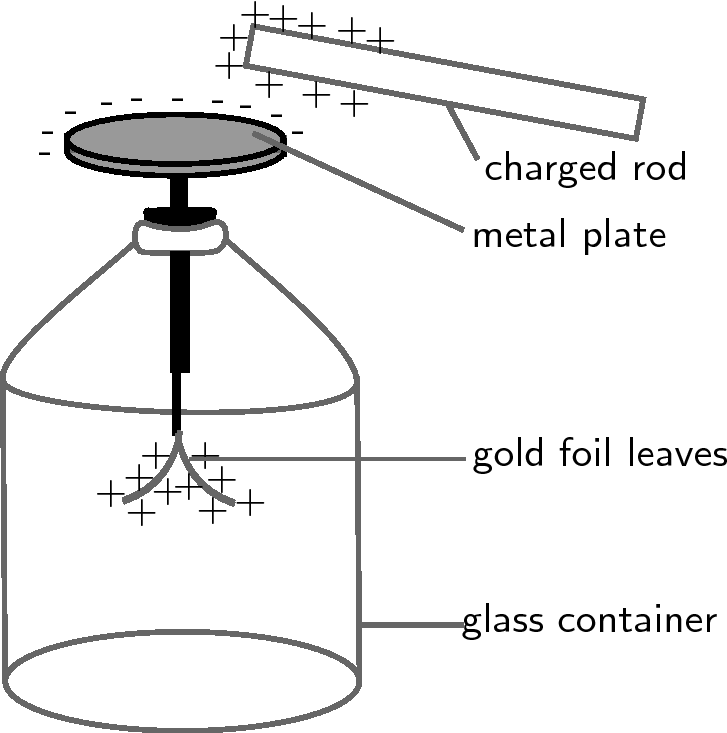
\includegraphics[height=300px]{col11305.imgs/m38781_PG10C8_009.png} % m38781;PG10C8\_009.png;;;6.0;8.5;
        
      \vspace{2pt}
    \vspace{.1in}
    
    \end{center}

 \end{figure}   

    \addtocounter{footnote}{-0}
    
        \par 
        \label{m38781*id200552}The electroscope detects charge in the following way: A charged object, like the positively charged rod in the picture, is brought close to (but not touching) the neutral metal plate of the electroscope. This causes negative charge in the gold foil, metal rod, and metal plate, to be attracted to the positive rod. Because the metal (gold is a metal too!) is a conductor, the charge can move freely from the foil up the metal rod and onto the metal plate. There is now more negative charge on the plate and more positive charge on the gold foil leaves. This is called \textsl{inducing} a charge on the metal plate. It is important to remember that the electroscope is still neutral (the total positive and negative charges are the same), the charges have just been induced to \textsl{move} to different parts of the instrument! The induced positive charge on the gold leaves forces them apart since like charges repel! This is how we can tell that the rod is charged. If the rod is now moved away from the metal plate, the charge in the electroscope will spread itself out evenly again and the leaves will fall down because there will no longer be an induced charge on them.\par 
        \label{m38781*uid12}
            \subsubsection{ Grounding}
            \nopagebreak
            
          
          \label{m38781*id200585}If you were to bring the charged rod close to the uncharged electroscope, and then you touched the metal plate with your finger at the same time, this would cause charge to flow up from the ground (the earth), through your body onto the metal plate. Connecting to the earth so charge flows is called \textbf{grounding}. The charge flowing onto the plate is opposite to the charge on the rod, since it is attracted to the charge on the rod. Therefore, for our picture, the charge flowing onto the plate would be negative. Now that charge has been added to the electroscope, it is no longer neutral, but has an excess of negative charge. Now if we move the rod away, the leaves will remain apart because they have an excess of negative charge and they repel each other. If we ground the electroscope again (this time without the charged rod nearby), the excess charge will flow back into the earth, leaving it neutral.\par 
          \label{m38781*id200601}
    \setcounter{subfigure}{0}


	\begin{figure}[H] % horizontal\label{m38781*id200605}
    \begin{center}
    \label{m38781*id200605!!!underscore!!!media}\label{m38781*id200605!!!underscore!!!printimage}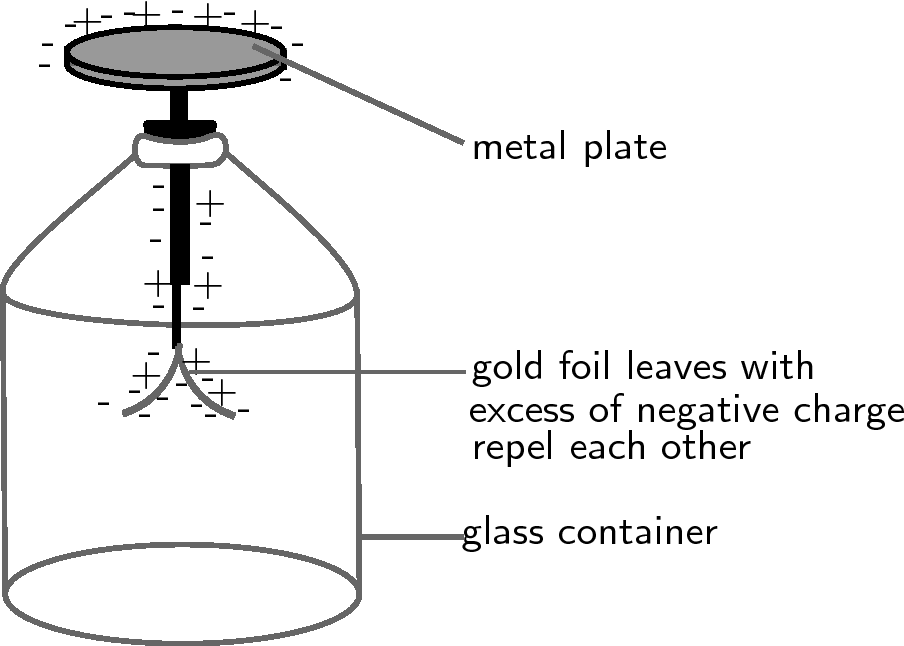
\includegraphics[width=300px]{col11305.imgs/m38781_PG10C8_010.png} % m38781;PG10C8\_010.png;;;6.0;8.5;
        
      \vspace{2pt}
    \vspace{.1in}
    
    \end{center}

 \end{figure}   

    \addtocounter{footnote}{-0}
    
          \par 
        
      
    
    

\label{m38781*fs-id1165908850940}
            \subsection{ Quantisation of Charge}
            \nopagebreak
            \label{m38781*eip-97}
            \subsubsection{ Unit of Charge}
            \nopagebreak
            

\label{m38781*id200658}Charge is measured in units called \textbf{coulombs (C)}. A coulomb of charge is a very large charge. In electrostatics we therefore often work with charge in microcoulombs (\begin{math}1\phantom{\rule{2pt}{0ex}}\mu \phantom{\rule{2pt}{0ex}}\mathrm{C}=1\ensuremath{\times}{10}^{-6}\phantom{\rule{2pt}{0ex}}\mathrm{C}\end{math}) and nanocoulombs (\begin{math}1\phantom{\rule{2pt}{0ex}}\phantom{\rule{2pt}{0ex}}\mathrm{nC}=1\ensuremath{\times}{10}^{-9}\phantom{\rule{2pt}{0ex}}\mathrm{C}\end{math}).
\par 

\label{m38781*eip-309}\vspace{.5cm} 
      
      \noindent
      \hspace*{-30pt}
\includegraphics[width=0.5in]{col11305.imgs/pspencil2.png}   \raisebox{25mm}{   
      \begin{mdframed}[linewidth=4, leftmargin=40, rightmargin=40]  
      \begin{exercise}
    \noindent\textbf{Exercise 15.5: Charge quantization}\label{m38781*eip-303}
  \label{m38781*eip-489}An object has an excess charge of \begin{math}-1,92\ensuremath{\times}{10}^{-17}\phantom{\rule{2pt}{0ex}}\mathrm{C}\end{math}. How many excess electrons does it have?
  \par 
\vspace{5pt}
\label{m38781*eip-671}\noindent\textbf{Solution to Exercise }
  \label{m38781*eip-id1170841837377}\begin{enumerate}[noitemsep, label=\textbf{Step} \textbf{\arabic*}. ] 
            \leftskip=20pt\rightskip=\leftskip\item  We are asked to determine a number of electrons based on a total charge. We know that charge is quantized and that electrons carry the base unit of charge which is \begin{math}-1,6\ensuremath{\times}{10}^{-19}\phantom{\rule{2pt}{0ex}}\mathrm{C}\end{math}.\item  As each electron carries the same charge the total charge must be made up of a certain number of electrons. To determine how many electrons we divide the total charge by the charge on a single electron:\label{m38781*id1166032483813}\nopagebreak\noindent{}\settowidth{\mymathboxwidth}{\begin{equation}
    \begin{array}{ccc}N=\frac{-1,92\ensuremath{\times}{10}^{-17}}{-1,6\ensuremath{\times}{10}^{-19}}\\ \phantom{x}=120\phantom{\rule{2pt}{0ex}}\mathrm{electrons}\end{array}\tag{15.3}
      \end{equation}
    }
    \typeout{Columnwidth = \the\columnwidth}\typeout{math as usual width = \the\mymathboxwidth}
    \ifthenelse{\lengthtest{\mymathboxwidth < \columnwidth}}{% if the math fits, do it again, for real
    \begin{equation}
    \begin{array}{ccc}N=\frac{-1,92\ensuremath{\times}{10}^{-17}}{-1,6\ensuremath{\times}{10}^{-19}}\\ \phantom{x}=120\phantom{\rule{2pt}{0ex}}\mathrm{electrons}\end{array}\tag{15.3}
      \end{equation}
    }{% else, if it doesn't fit
    \setlength{\mymathboxwidth}{\columnwidth}
      \addtolength{\mymathboxwidth}{-48pt}
    \par\vspace{12pt}\noindent\begin{minipage}{\columnwidth}
    \parbox[t]{\mymathboxwidth}{\large\begin{math}
    N=\frac{-1,92\ensuremath{\times}{10}^{-17}}{-1,6\ensuremath{\times}{10}^{-19}}\phantom{x}=120\phantom{\rule{2pt}{0ex}}\mathrm{electrons}\end{math}}\hfill
    \parbox[t]{48pt}{\raggedleft 
    (15.3)}
    \end{minipage}\vspace{12pt}\par
    }% end of conditional for this bit of math
    \typeout{math as usual width = \the\mymathboxwidth}
    \end{enumerate}
        


    \end{exercise}
    \end{mdframed}
    }
    \noindent
  \par
            \label{m38781*eip-409}\vspace{.5cm} 
      
      \noindent
      \hspace*{-30pt}
\includegraphics[width=0.5in]{col11305.imgs/pspencil2.png}   \raisebox{25mm}{   
      \begin{mdframed}[linewidth=4, leftmargin=40, rightmargin=40]  
      \begin{exercise}
    \noindent\textbf{Exercise 15.6: Conservation of charge - 1}\label{m38781*eip-30443}
\label{m38781*id1166015493890}Two identical, metal spheres have different charges. Sphere 1 has a charge of \begin{math}-9,6\ensuremath{\times}{10}^{-18}\phantom{\rule{2pt}{0ex}}\mathrm{C}\end{math}. Sphere 2 has 30 excess electrons. If the two spheres are brought into contact and then separated, what charge will each have? How many electrons does this correspond to?\par 
\vspace{5pt}
\label{m38781*eip-67221}\noindent\textbf{Solution to Exercise }
  \label{m38781*eip-id11737377}\begin{enumerate}[noitemsep, label=\textbf{Step} \textbf{\arabic*}. ] 
            \leftskip=20pt\rightskip=\leftskip\item \newline
     We need to determine what will happen to the charge when the spheres touch. They are metal spheres so we know they will be conductors. This means that the charge is able to move so when they touch it is possible for the charge on each sphere to change. We know that charge will redistribute evenly across the two spheres because of the forces between the charges. We need to know the charge on each sphere, we have been given one.\item \newline
     This problem is similar to the earlier worked example. This time we have to determine the total charge given a certain number of electrons. We know that charge is quantized and that electrons carry the base unit of charge which is \begin{math}-1,6\ensuremath{\times}{10}^{-19}\phantom{\rule{2pt}{0ex}}\mathrm{C}\end{math}. The total charge will therefore be:
\label{m38781*id6322}\nopagebreak\noindent{}\settowidth{\mymathboxwidth}{\begin{equation}
    \begin{array}{ccc}{Q}_{2}=30\ensuremath{\times}-1,6\ensuremath{\times}{10}^{-19}\phantom{\rule{2pt}{0ex}}\mathrm{C}\\ \phantom{x}=4,8\ensuremath{\times}{10}^{-18}\phantom{\rule{2pt}{0ex}}\mathrm{C}\end{array}\tag{15.4}
      \end{equation}
    }
    \typeout{Columnwidth = \the\columnwidth}\typeout{math as usual width = \the\mymathboxwidth}
    \ifthenelse{\lengthtest{\mymathboxwidth < \columnwidth}}{% if the math fits, do it again, for real
    \begin{equation}
    \begin{array}{ccc}{Q}_{2}=30\ensuremath{\times}-1,6\ensuremath{\times}{10}^{-19}\phantom{\rule{2pt}{0ex}}\mathrm{C}\\ \phantom{x}=4,8\ensuremath{\times}{10}^{-18}\phantom{\rule{2pt}{0ex}}\mathrm{C}\end{array}\tag{15.4}
      \end{equation}
    }{% else, if it doesn't fit
    \setlength{\mymathboxwidth}{\columnwidth}
      \addtolength{\mymathboxwidth}{-48pt}
    \par\vspace{12pt}\noindent\begin{minipage}{\columnwidth}
    \parbox[t]{\mymathboxwidth}{\large\begin{math}
    {Q}_{2}=30\ensuremath{\times}-1,6\ensuremath{\times}{10}^{-19}\phantom{\rule{2pt}{0ex}}\mathrm{C}\phantom{x}=4,8\ensuremath{\times}{10}^{-18}\phantom{\rule{2pt}{0ex}}\mathrm{C}\end{math}}\hfill
    \parbox[t]{48pt}{\raggedleft 
    (15.4)}
    \end{minipage}\vspace{12pt}\par
    }% end of conditional for this bit of math
    \typeout{math as usual width = \the\mymathboxwidth}
    \item \newline
     As the spheres are identical in material, size and shape the charge will redistribute across the two spheres so that it is shared evenly. Each sphere will have half of the total charge:
\label{m38781*id3231}\nopagebreak\noindent{}\settowidth{\mymathboxwidth}{\begin{equation}
    \begin{array}{ccc}Q=\frac{{Q}_{1}+{Q}_{2}}{2}\\ \phantom{x}=\frac{-9.6\ensuremath{\times}{10}^{-18}+\left(-4,8\ensuremath{\times}{10}^{-18}\right)}{2}\\ \phantom{x}=7,2\ensuremath{\times}{10}^{-18}\phantom{\rule{2pt}{0ex}}\mathrm{C}\end{array}\tag{15.5}
      \end{equation}
    }
    \typeout{Columnwidth = \the\columnwidth}\typeout{math as usual width = \the\mymathboxwidth}
    \ifthenelse{\lengthtest{\mymathboxwidth < \columnwidth}}{% if the math fits, do it again, for real
    \begin{equation}
    \begin{array}{ccc}Q=\frac{{Q}_{1}+{Q}_{2}}{2}\\ \phantom{x}=\frac{-9.6\ensuremath{\times}{10}^{-18}+\left(-4,8\ensuremath{\times}{10}^{-18}\right)}{2}\\ \phantom{x}=7,2\ensuremath{\times}{10}^{-18}\phantom{\rule{2pt}{0ex}}\mathrm{C}\end{array}\tag{15.5}
      \end{equation}
    }{% else, if it doesn't fit
    \setlength{\mymathboxwidth}{\columnwidth}
      \addtolength{\mymathboxwidth}{-48pt}
    \par\vspace{12pt}\noindent\begin{minipage}{\columnwidth}
    \parbox[t]{\mymathboxwidth}{\large\begin{math}
    Q=\frac{{Q}_{1}+{Q}_{2}}{2}\phantom{x}=\frac{-9.6\ensuremath{\times}{10}^{-18}+\left(-4,8\ensuremath{\times}{10}^{-18}\right)}{2}\phantom{x}=7,2\ensuremath{\times}{10}^{-18}\phantom{\rule{2pt}{0ex}}\mathrm{C}\end{math}}\hfill
    \parbox[t]{48pt}{\raggedleft 
    (15.5)}
    \end{minipage}\vspace{12pt}\par
    }% end of conditional for this bit of math
    \typeout{math as usual width = \the\mymathboxwidth}
    
 So each sphere now has: 
\label{m38781*id61212}\nopagebreak\noindent{}\settowidth{\mymathboxwidth}{\begin{equation}
    7,2\ensuremath{\times}{10}^{-18}\phantom{\rule{2pt}{0ex}}\mathrm{C}\tag{15.6}
      \end{equation}
    }
    \typeout{Columnwidth = \the\columnwidth}\typeout{math as usual width = \the\mymathboxwidth}
    \ifthenelse{\lengthtest{\mymathboxwidth < \columnwidth}}{% if the math fits, do it again, for real
    \begin{equation}
    7,2\ensuremath{\times}{10}^{-18}\phantom{\rule{2pt}{0ex}}\mathrm{C}\tag{15.6}
      \end{equation}
    }{% else, if it doesn't fit
    \setlength{\mymathboxwidth}{\columnwidth}
      \addtolength{\mymathboxwidth}{-48pt}
    \par\vspace{12pt}\noindent\begin{minipage}{\columnwidth}
    \parbox[t]{\mymathboxwidth}{\large\begin{math}
    7,2\ensuremath{\times}{10}^{-18}\phantom{\rule{2pt}{0ex}}\mathrm{C}\end{math}}\hfill
    \parbox[t]{48pt}{\raggedleft 
    (15.6)}
    \end{minipage}\vspace{12pt}\par
    }% end of conditional for this bit of math
    \typeout{math as usual width = \the\mymathboxwidth}
     of charge.\item \newline
     We know that charge is quantized and that electrons carry the base unit of charge which is \begin{math}-1,6\ensuremath{\times}{10}^{-19}\phantom{\rule{2pt}{0ex}}\mathrm{C}\end{math}.\item \newline
     As each electron carries the same charge the total charge must be made up of a certain number of electrons. To determine how many electrons we divide the total charge by the charge on a single electron:
\label{m38781*id5121}\nopagebreak\noindent{}\settowidth{\mymathboxwidth}{\begin{equation}
    \begin{array}{ccc}N=\frac{-7,2\ensuremath{\times}{10}^{-18}}{-1,6\ensuremath{\times}{10}^{-19}}\\ \phantom{x}=45\phantom{\rule{2pt}{0ex}}\mathrm{electrons}\end{array}\tag{15.7}
      \end{equation}
    }
    \typeout{Columnwidth = \the\columnwidth}\typeout{math as usual width = \the\mymathboxwidth}
    \ifthenelse{\lengthtest{\mymathboxwidth < \columnwidth}}{% if the math fits, do it again, for real
    \begin{equation}
    \begin{array}{ccc}N=\frac{-7,2\ensuremath{\times}{10}^{-18}}{-1,6\ensuremath{\times}{10}^{-19}}\\ \phantom{x}=45\phantom{\rule{2pt}{0ex}}\mathrm{electrons}\end{array}\tag{15.7}
      \end{equation}
    }{% else, if it doesn't fit
    \setlength{\mymathboxwidth}{\columnwidth}
      \addtolength{\mymathboxwidth}{-48pt}
    \par\vspace{12pt}\noindent\begin{minipage}{\columnwidth}
    \parbox[t]{\mymathboxwidth}{\large\begin{math}
    N=\frac{-7,2\ensuremath{\times}{10}^{-18}}{-1,6\ensuremath{\times}{10}^{-19}}\phantom{x}=45\phantom{\rule{2pt}{0ex}}\mathrm{electrons}\end{math}}\hfill
    \parbox[t]{48pt}{\raggedleft 
    (15.7)}
    \end{minipage}\vspace{12pt}\par
    }% end of conditional for this bit of math
    \typeout{math as usual width = \the\mymathboxwidth}
    \end{enumerate}
        


    \end{exercise}
    \end{mdframed}
    }
    \noindent
  
\label{m38781*cid9}
            \subsection{ Summary}
            \nopagebreak
            
      
      \label{m38781*id201947}\begin{enumerate}[noitemsep, label=\textbf{\arabic*}. ] 
            \label{m38781*uid14}\item Objects can be \textbf{positively} charged, \textbf{negatively} charged or \textbf{neutral}.
\label{m38781*uid15}\item Objects that are neutral have equal numbers of positive and negative charge.
\label{m38781*uid16}\item Unlike charges are attracted to each other and like charges are repelled from each other.
\label{m38781*uid17}\item Charge is neither created nor destroyed, it can only be transferred.
\label{m38781*uid18}\item Charge is measured in coulombs (C).
\label{m38781*uid19}\item Conductors allow charge to move through them easily.
\label{m38781*uid20}\item Insulators do not allow charge to move through them easily.
\end{enumerate}
        \label{m38781*eip-152}The following presentation is a summary of the work covered in this chapter. Note that the last two slides are not needed for exam purposes, but are included for general interest.\newline
    

    \setcounter{subfigure}{0}


	\begin{figure}[H] % horizontal\label{m38781*slidesharefigure}
    
    \label{m38781*slidesharemedia}\label{m38781*slideshareflash}\raisebox{-5 pt}{ 
\includegraphics[width=0.5cm]{col11305.imgs/summary_www.png}} { (Presentation:  P10073 )}
      
      \vspace{2pt}
    \vspace{.1in}
    
    

 \end{figure}   

    \addtocounter{footnote}{-0}
    \par 
    
    \label{m38781*cid10}
            \subsection{ End of chapter exercise}
            \nopagebreak
            
      
      \label{m38781*id202059}\begin{enumerate}[noitemsep, label=\textbf{\arabic*}. ] 
            \label{m38781*uid21}\item What are the two types of charge called?\newline
            
\label{m38781*uid22}\item Provide evidence for the existence of two types of charge.\newline
            
\label{m38781*uid23}\item Fill in the blanks: The electrostatic force between like charges is  \uline{\hspace{10ex}}
 while the electrostatic force between opposite charges is  \uline{\hspace{10ex}}
.\newline
            
\label{m38781*uid24}\item I have two positively charged metal balls placed 2 m apart.
\label{m38781*id202122}\begin{enumerate}[noitemsep, label=\textbf{\alph*}. ] 
            \label{m38781*uid25}\item Is the electrostatic force between the balls attractive or repulsive?
\label{m38781*uid26}\item If I now move the balls so that they are 1 m apart, what happens to the strength of the electrostatic force between them?
\end{enumerate}
        \newline
            \label{m38781*uid27}\item I have 2 charged spheres each hanging from string as shown in the picture below.

    \setcounter{subfigure}{0}


	\begin{figure}[H] % horizontal\label{m38781*id202166}
    \begin{center}
    \label{m38781*id202166!!!underscore!!!media}\label{m38781*id202166!!!underscore!!!printimage}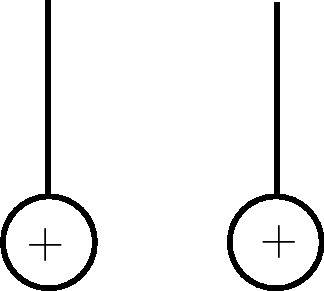
\includegraphics[width=300px]{col11305.imgs/m38781_PG10C8_012.png} % m38781;PG10C8\_012.png;;;6.0;8.5;
        
      \vspace{2pt}
    \vspace{.1in}
    
    \end{center}

 \end{figure}   

    \addtocounter{footnote}{-0}
    
Choose the correct answer from the options below:
The spheres will
\label{m38781*id202176}\begin{enumerate}[noitemsep, label=\textbf{\alph*}. ] 
            \label{m38781*uid28}\item swing towards each other due to the attractive electrostatic force between them.
\label{m38781*uid29}\item swing away from each other due to the attractive electrostatic force between them.
\label{m38781*uid30}\item swing towards each other due to the repulsive electrostatic force between them.
\label{m38781*uid31}\item swing away from each other due to the repulsive electrostatic force between them.
\end{enumerate}
        \newline
            \label{m38781*uid32}\item Describe how objects (insulators) can be charged by contact or rubbing.\newline
            
\label{m38781*uid33}\item You are given a perspex ruler and a piece of cloth.
\label{m38781*id202255}\begin{enumerate}[noitemsep, label=\textbf{\alph*}. ] 
            \label{m38781*uid34}\item How would you charge the perspex ruler?
\label{m38781*uid35}\item Explain how the ruler becomes charged in terms of charge.
\label{m38781*uid36}\item How does the charged ruler attract small pieces of paper?
\end{enumerate}
        \newline
            \label{m38781*uid37}\item [IEB 2005/11 HG] An uncharged hollow metal sphere is placed on an insulating stand. A positively charged rod is brought up to touch the hollow metal sphere at P as shown in the diagram below. It is then moved away from the sphere.

    \setcounter{subfigure}{0}


	\begin{figure}[H] % horizontal\label{m38781*id202314}
    \begin{center}
    \label{m38781*id202314!!!underscore!!!media}\label{m38781*id202314!!!underscore!!!printimage}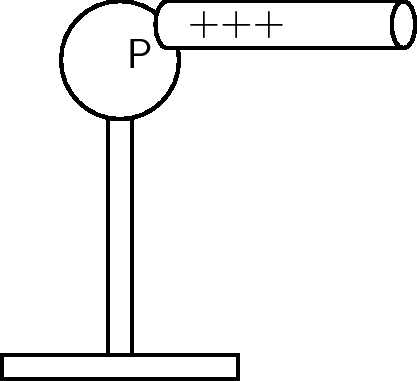
\includegraphics[width=300px]{col11305.imgs/m38781_PG10C8_013.png} % m38781;PG10C8\_013.png;;;6.0;8.5;
        
      \vspace{2pt}
    \vspace{.1in}
    
    \end{center}

 \end{figure}   

    \addtocounter{footnote}{-0}
    
Where is the excess charge distributed on the sphere after the rod
has been removed?
\label{m38781*id202325}\begin{enumerate}[noitemsep, label=\textbf{\alph*}. ] 
            \label{m38781*uid38}\item It is still located at point P where the rod touched the sphere.
\label{m38781*uid39}\item It is evenly distributed over the outer surface of the hollow sphere.
\label{m38781*uid40}\item It is evenly distributed over the outer and inner surfaces of the hollow sphere.
\label{m38781*uid41}\item No charge remains on the hollow sphere.
\end{enumerate}
        \newline
            \label{m38781*uid42}\item What is the process called where molecules in an uncharged object are caused to align in a particular direction due to an external charge?\newline
            
\label{m38781*uid43}\item Explain how an uncharged object can be attracted to a charged object. You should use diagrams to illustrate your answer.\newline
            
\label{m38781*uid44}\item Explain how a stream of water can be attracted to a charged rod.\newline
            
\item An object has an excess charge of 
\begin{math}-8,6\ensuremath{\times}{10}^{-18}\phantom{\rule{2pt}{0ex}}\mathrm{C}\end{math}. How many excess electrons does it have?\newline
            \item An object has an excess of 235 electrons. What is the charge on the object?\newline
            \item An object has an excess of 235 protons. What is the charge on the object?\newline
            \item Two identical, metal spheres have different charges. Sphere 1 has a charge of 
\begin{math}-4,8\ensuremath{\times}{10}^{-18}\phantom{\rule{2pt}{0ex}}\mathrm{C}\end{math}. Sphere 2 has 60 excess electrons. If the two spheres are brought into contact and then separated, what charge will each have? How many electrons does this correspond to?\newline
            \item Two identical, insulated spheres have different charges. Sphere 1 has a charge of 
\begin{math}-96\ensuremath{\times}{10}^{-18}\phantom{\rule{2pt}{0ex}}C\end{math}. Sphere 2 has 60 excess electrons. If the two spheres are brought into contact and then separated, what charge will each have? \newline
            \item Two identical, metal spheres have different charges. Sphere 1 has a charge of 
\begin{math}-4,8\ensuremath{\times}{10}^{-18}\phantom{\rule{2pt}{0ex}}\mathrm{C}\end{math}. Sphere 2 has 30 excess protons. If the two spheres are brought into contact and then separated, what charge will each have? How many electrons or protons does this correspond to?\newline
            \end{enumerate}
        
    
  \label{m38781**end}
          
       
    
  \label{464e844ca5615087ea89d9d95dd9a43a**end}
    
\par \raisebox{-5 pt}{
\includegraphics[width=0.5cm]{col11305.imgs/summary_www.png}} Find the answers with the shortcodes:
 \par \begin{tabular}[h]{cccccc}
 (1.) lqs  &  (2.) lqo  &  (3.) lqA  &  (4.) lqG  &  (5.) lqf  &  (6.) lqw  &  (7.) lqv  &  (8.) lqd  &  (9.) lqp  &  (10.) la2  &  (11.) lqP  &  (12.) lTf  &  (13.) lTG  &  (14.) lT7  &  (15.) lTA  &  (16.) lTo  &  (17.) lTs  & \end{tabular}



